%FOR PDFLATEX USE ONLY
\documentclass[a4paper,12pt]{article}

\usepackage{amssymb,amsmath} %math symbols

\usepackage[margin=2cm]{geometry} %paper geometry

\usepackage[T1, T2A]{fontenc}

\usepackage[utf8]{inputenc} %allows unicode (including russian) source file
\usepackage[russian]{babel} %docment in russian-style
\usepackage[utf8]{inputenc}
%\usepackage[unicode]{hyperref} %links inside of the text
\usepackage[pdftex]{graphicx} %includegraphics pictures
\usepackage{cmlgc} %bold text

\usepackage{array} %arrays

%\usepackage{wrapfig}
%\usepackage{array}
%\usepackage{lipsum}
%\usepackage{esvect}
%\usepackage{hyperref}

\usepackage{amsmath}
\usepackage{amssymb}
\usepackage{mathtools}
\usepackage{mathtext}

\usepackage{subfig}
%\usepackage{calc}
%\usepackage{pgfplots,tikz,circuitikz}
%\usepackage{tkz-euclide}
\usepackage{booktabs}
\usepackage{multirow}

\begin{document}

\begin{center}
  \LARGE{Работа 2.2.1}\\[0.2cm]
  \LARGE{Исследование взаимной диффузии газов}\\[0.2cm]
  \large{Малиновский Владимир}\\[0.2cm]
  \normalsize{\texttt{galqiwi@galqiwi.ru}}
\end{center}

\textbf{Цель работы:} 1) регистрация зависимости концентрации гелия в воздухе от времени с помощью датчиков теплопроводности при разных начальных давлениях смеси газов; 2) определение коэффициента диффузии по результатам измерений

\textbf{В работе используются:} измерительная установка; форвакуумный насос; баллон с газом (гелий); манометр; источник питания; магазин сопротивлений; гальванометр; секундомер.

\section*{Описание работы}
В этой работе измеряется зависимость разности концентрации гелия в двух сосудах $V_1$ и $V_2$ от времени с помощью датчиков теплопроводности $D_1$ и $D_2$ в этих сосудах. Эта зависимость должна быть экспоненциальной:
$$n_1 - n_2 = (n_1 - n_2)_0e^{-t/\tau},$$
из чего можно найти $\tau = 1 / A$.\\
Также известно, что $\tau$ зависит от коэффициента диффузии $D$, как
$$\tau = \frac{V_1V_2}{V_1 + V_2} \frac{l}{SD},$$
где S -- площадь сечения, L -- длина канала между $V_1$ и $V_2$.\\
В свою очередь, $D\sim1/P$, где $P$ -- давление внутри сосуда. Эту закономерность нам предстоит проверить.
\begin{center}
	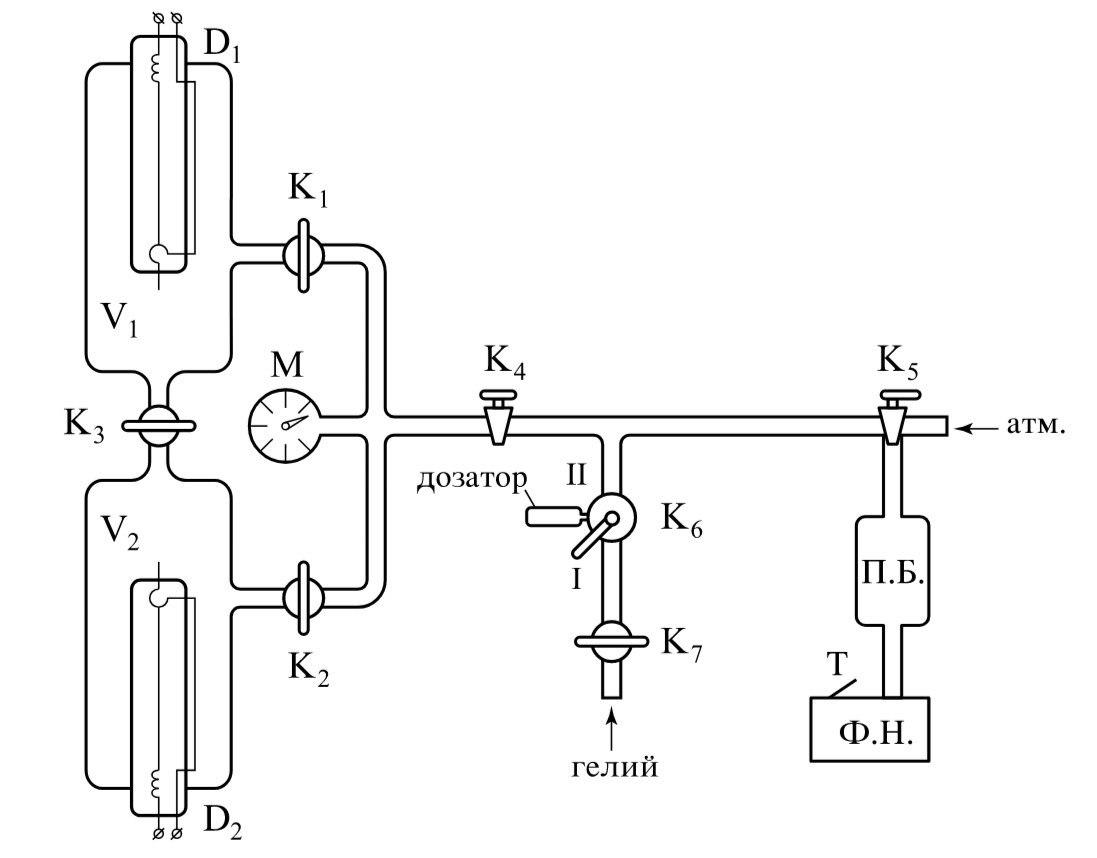
\includegraphics[width=0.80\textwidth]{setup.png}
\end{center}
\newpage
\section*{Ход работы, результаты и обработка}
\subsection*{1-3}
Откроем кран $K_4$, включим насос и откачаем установку до давления $\sim0.1\,\text{торр}$, оставив насос работать на 3 минуты.
\subsection*{4}
Сбалансируем мост.\\
Напустим воздух до рабочего давления $\sim40\,\text{торр}$, а потом будем менять сопротивление в мосту так, чтобы показания гальванометра были около нуля.
\subsection*{5}
Когда мост сбалансирован -- можно приступать к основной работе.
\begin{enumerate}
	\item Откачаем установку до $\sim0.1\,\text{торр}$
	\item Закроем краны $K_2$ и $K_3$, изолируя объем $V_2$.
	\item Пустим немного гелия до давления порядка $10\%$ от рабочего.
	\item Откроем кран $K_2$ и закроем $K_1$, изолируя объем $V_1$
	\item Заполним объем $V_2$ до давления $\sim 1.5P_\text{раб}$
	\item Откроем кран $K_1$ для того, чтобы воздух проник в объем $V_1$
\end{enumerate}
\subsection*{6}
Откроем кран $K_3$ и начнем измерять зависимость показаний гальванометра от времени
\subsection*{7}
Повторим пункты 3-6 для других рабочих давлений
\subsection*{8}
Построим зависимость $ln(V/V_0)$ -- логарифма напряжения на гальванометре ($V_0 = 1\text{мВ}$) от $t$. Эти графики линейные, что соответствует теории. Из МНК найдем $A$ -- их графики наклона, из которых вычислим $D$.
\begin{center}
	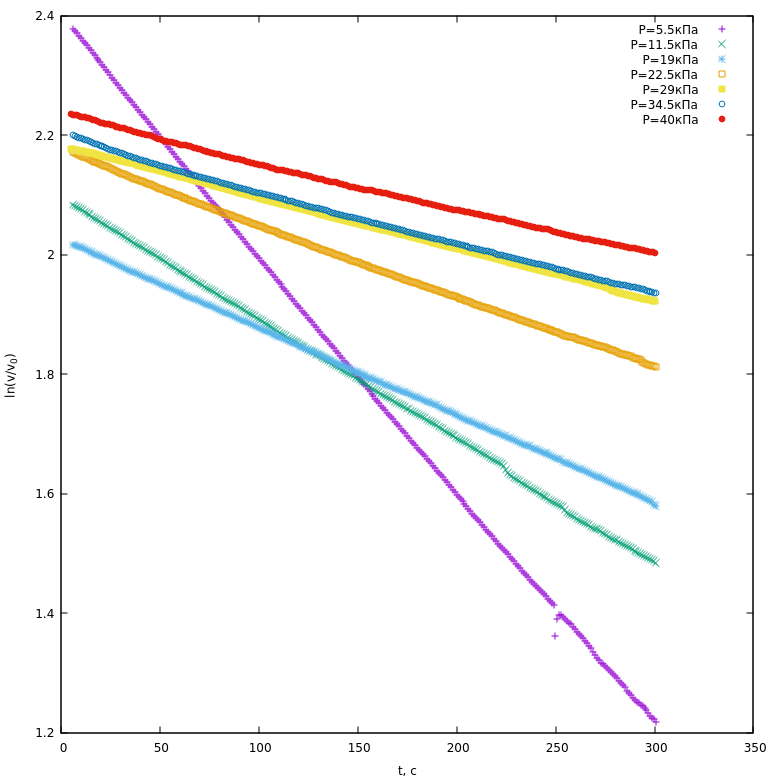
\includegraphics[width=0.80\textwidth]{plot_0.png}
\end{center}

\begin{center}
\begin{tabular}{|c|c|c|c|c|c|c|c|}\hline
$P_\text{раб},\,\text{кПа}$&$A, \text{кс}^{-1}$&$10\,\text{кПа}/P_\text{раб}$&$\Delta 10\,\text{кПа}/P_\text{раб}$
&$D, \text{cм}^2/\text{с}$&$\Delta D, \text{cм}^2/\text{с}$
\\ \hline
$5.4$&$3.945$&$1.86$&$0.08$&$7$&$1$\\ \hline
$11.3$&$2.041$&$0.89$&$0.02$&$3.9$&$0.5$\\ \hline
$18.6$&$1.464$&$0.537$&$0.007$&$2.8$&$0.4$\\ \hline
$22.1$&$1.200$&$0.454$&$0.005$&$2.3$&$0.3$\\ \hline
$28.4$&$0.865$&$0.352$&$0.003$&$1.6$&$0.2$\\ \hline
$33.8$&$0.871$&$0.296$&$0.002$&$1.6$&$0.2$\\ \hline
$39.2$&$0.779$&$0.2551$&$0.0016$&$1.5$&$0.2$\\ \hline
\end{tabular}
\end{center}
$$\Delta P_\text{раб}=0.25\,\,\text{кПа},\,\,\Delta A=0.001\, \text{кс}^{-1}.$$

$$V_1=V_2=V=(420\pm10)\,\text{мл},\,l/S=(9.0\pm0.1)\,1/\text{см}$$

\subsubsection*{погрешности}
$$\delta D = \delta \tau + \delta (l/S) + \delta V$$
$$\delta (1/P) = \delta P$$

\subsection*{9}
Если построить график зависимости $D$ от $1/P_\text{раб}$, то он получается линейным, что согласуется с теорией.
Из МНК следует, что при $10\,\text{кПа}/P = 0.1$,
$$D_\text{атм} = (0.91\pm 0.08) \text{см}^2/\text{с}.$$
Посчитаем полную погрешность:
$$\Delta D = \sqrt{\Delta D_\text{стат}^2 + <\Delta D>^2}$$
$$D_\text{атм} = (0.9 \pm 0.4) \text{см}^2/\text{с}.$$
Табличное значение
$$D_\text{табл} = 0.83 \text{см}^2/\text{с}$$
\begin{center}
	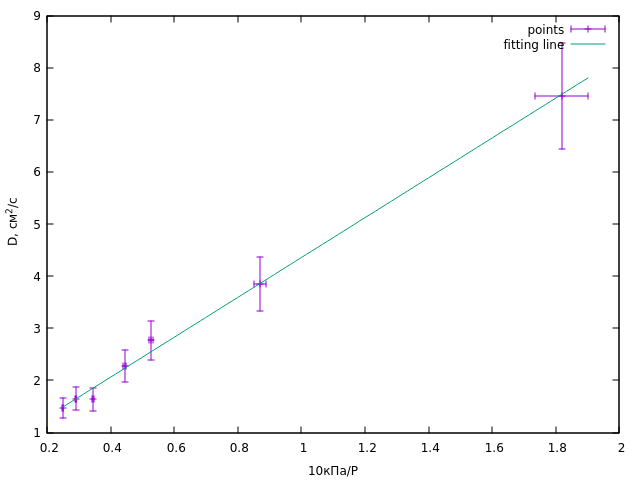
\includegraphics[width=0.80\textwidth]{plot_1.png}
\end{center}
\subsection*{10}
Из значений $D$, можно найти $\lambda = \frac{3D}{\sqrt{3RT/\mu}}$ и $\sigma = \frac{\sqrt{\frac{3RT}{\mu}}}{3\frac{p}{RT}D} \frac{1}{N_\text{а}}$ ($T=300\text{К}$ (вообще, нет, но у $D$ большая погрешность, так что неточность T незначительна)):

$$\lambda = (200\pm90)\text{нм},\,\sigma = (0.21\pm0.09)\text{нм}^2,$$
что похоже на правду.
\section*{Вывод}
Мы научились измерять разницу концентраций в процессе диффузии газов от времени. Благодаря этому, мы получили зависимость $D$ от $P$ с величинами, близкими к табличным. К сожалению, погрешность $D$ была высока (так как погрешность $l/S$ была $1/9$), и не получилось получить точное значение $D$ при комнатной температуре. Полученное значение все же сходится с табличным, учитывая погрешность. Полученные из $D$ значения $\lambda$ и $\sigma$ при атмосферном давлении похожи на правду, и сходятся с табичными ровно настолько, насколько с табличными значениями сходится $D$.


\end{document}


\lipsum[1-4]
\begin{wrapfigure}{R}{5cm}
\centering
\includegraphics[width=0.20\textwidth]{rd.png}
\caption{1}
\end{wrapfigure}
\lipsum[1-6]


\begin{figure}[h]
\begin{center}$
\begin{array}{cccc}
\includegraphics[width=0.20\textwidth]{rd.png}&
\includegraphics[width=0.20\textwidth]{rd.png}&
\includegraphics[width=0.20\textwidth]{rd.png}&
\includegraphics[width=0.20\textwidth]{rd.png}\\
(1) & (2) & (3) & (4)
\end{array}$
\end{center}
\end{figure}
